\chapter{Implementation}
\graphicspath{{Chapter4/Figs/}{Chapter4/Figs/}}

The implementation details of creating the software components for the NIP of IDUN are covered in this chapter, along with key events in the empirical software engineering process like the recognition of novelty and the requirement for a N/CI definition.

\section{Timeline}
\label{chapter4-timeline}

Procedures enlisted in the project stages presented in \autoref{chapter3-project-stages} are a good guide for project implementation, but in the end, such plans run in unexpected ways. As a result, researching and implementing a non-trivial system such as a N/CI requires a high level of agility.

The effective timeline at the time of writing is shown in \autoref{fig:implementation-timeline}. It includes the previously mentioned project stages but is differently structured as initially described. \autoref{tab:special-project-stages} explains why some project stages were completed differently than initially assumed.

\begin{figure}[!ht]
  \centering
  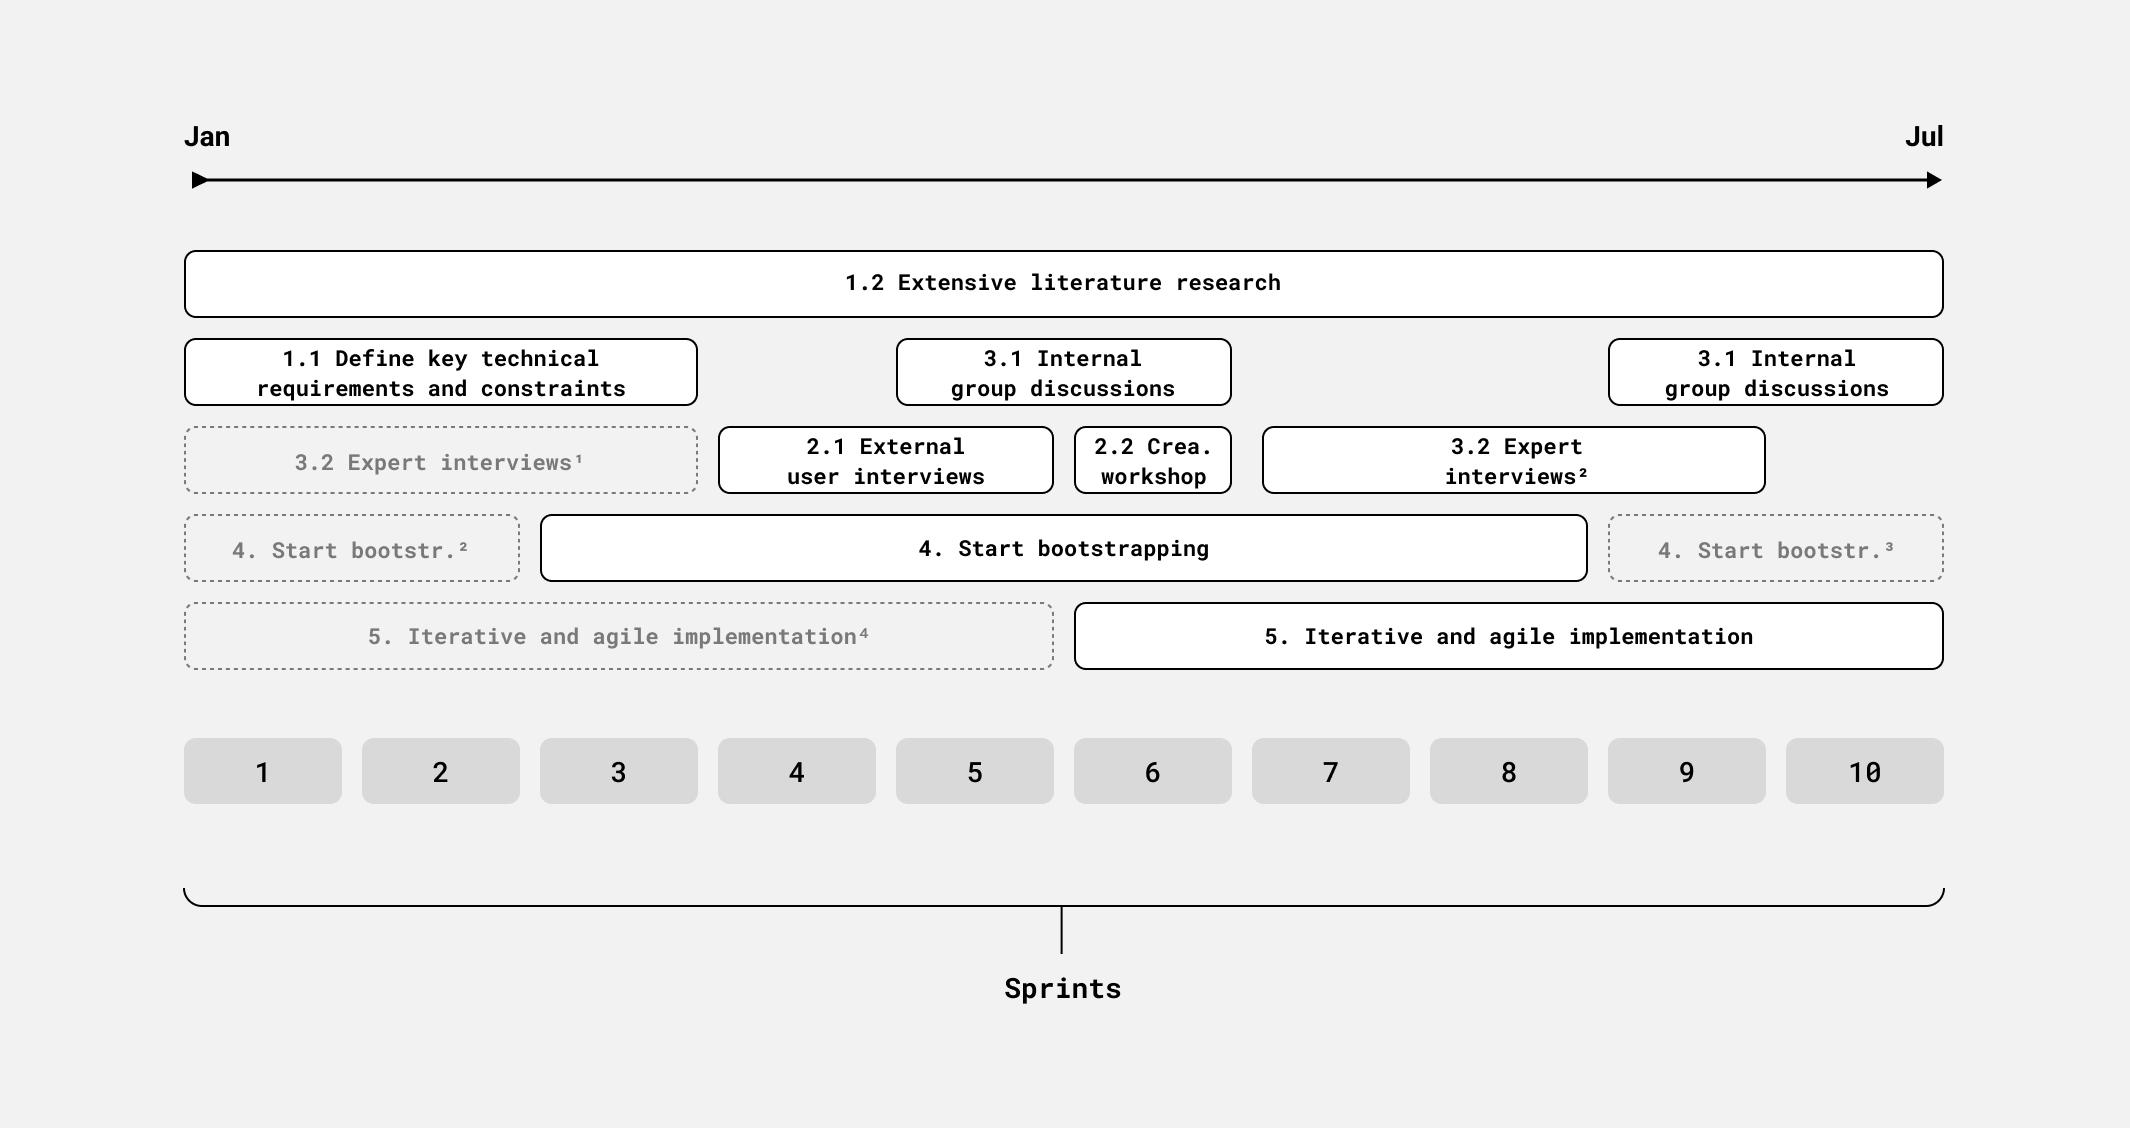
\includegraphics[width=\linewidth]{implementation-timeline.png}
  \caption{Effective timeline of the last ten sprints with project stages in white and specifically planned stages outlined in grey.}
  \label{fig:implementation-timeline}
\end{figure}

\begin{table}[ht]
  \centering
  \resizebox{\textwidth}{!}{%
    \begin{tabular}{
        >{\columncolor[HTML]{FFFFFF}}l l}
      \cellcolor[HTML]{000000}{\color[HTML]{FFFFFF} Special stage}                                                                               &
      \cellcolor[HTML]{000000}{\color[HTML]{FFFFFF} Description}                                                                                                                                                                                                                                                                                                                                                                                \\ \hline
      \multicolumn{1}{|l|}{\cellcolor[HTML]{FFFFFF}\textbf{\begin{tabular}[c]{@{}l@{}}[1] 3.2 Expert\\ interviews\end{tabular}}}                 &
      \multicolumn{1}{l|}{\begin{tabular}[c]{@{}l@{}}The author was able to use the first expert discussions in advance thanks to the help of one\\ of the sales staff's networks. The experts were Nuvibit's experienced enterprise cloud and\\ solution architects. The first topics were strictly technical in nature, focusing on medium-\\ term technological decisions in the context of the company and the timetable.\end{tabular}}     \\ \hline
      \multicolumn{1}{|l|}{\cellcolor[HTML]{FFFFFF}\textbf{\begin{tabular}[c]{@{}l@{}}[2] 4. Start\\ bootstrapping\end{tabular}}}                &
      \multicolumn{1}{l|}{\begin{tabular}[c]{@{}l@{}}This special stage describes the phase in which the author established more organisational\\ structures, such as a professional Scrum or GitHub setup. Furthermore, the time was used\\ to create a more professional AWS organisational setup with various organisational units,\\ as described in the AWS Best Practice Guide \citep{blackham_best_2020}.\end{tabular}}                  \\ \hline
      \multicolumn{1}{|l|}{\cellcolor[HTML]{FFFFFF}\textbf{\begin{tabular}[c]{@{}l@{}}[3] 4. Start\\ bootstrapping\end{tabular}}}                &
      \multicolumn{1}{l|}{\begin{tabular}[c]{@{}l@{}}Since the creation of two different Python SDKs (as discussed later in this chapter), more\\ bootstrapping tasks were due at the very end of the given time frame, mostly including\\ the setup of a privately installable Python package and SDK-specific quality\\ assurance pipelines and automations.\end{tabular}}                                                                    \\ \hline
      \multicolumn{1}{|l|}{\cellcolor[HTML]{FFFFFF}\textbf{\begin{tabular}[c]{@{}l@{}}[4] 5. Iterative and\\ agile implementation\end{tabular}}} &
      \multicolumn{1}{l|}{\begin{tabular}[c]{@{}l@{}}Iterative and agile implementation began as soon as needed, without waiting for the design\\ process to be completed (i.e. avoiding a waterfall process). Prior to gaining insights from the \\ design process, time was spent on everything else, such as evaluating technologies, further\\ bootstrapping, first example codebases, or maintaining the old codebase a bit.\end{tabular}} \\ \hline
    \end{tabular}%
  }
  \vspace{10pt}
  \caption{Special project stages in the effective schedule as shown in \autoref{fig:implementation-timeline} and their explanation of why they took place there.}
  \vspace{-5pt}
  \label{tab:special-project-stages}
\end{table}

\newpage

Several key events occurred during the implementation that shaped the future course of the project and research. This was primarily due to initially unplanned early expert discussions or uncertainties in the requirements as the user-centred design process was still being prepared. These key events are overlaid with the effective project plan as shown in \autoref{fig:implementation-timeline-key-events}. These three green key events are the most influential key events.

\begin{figure}[!ht]
  \centering
  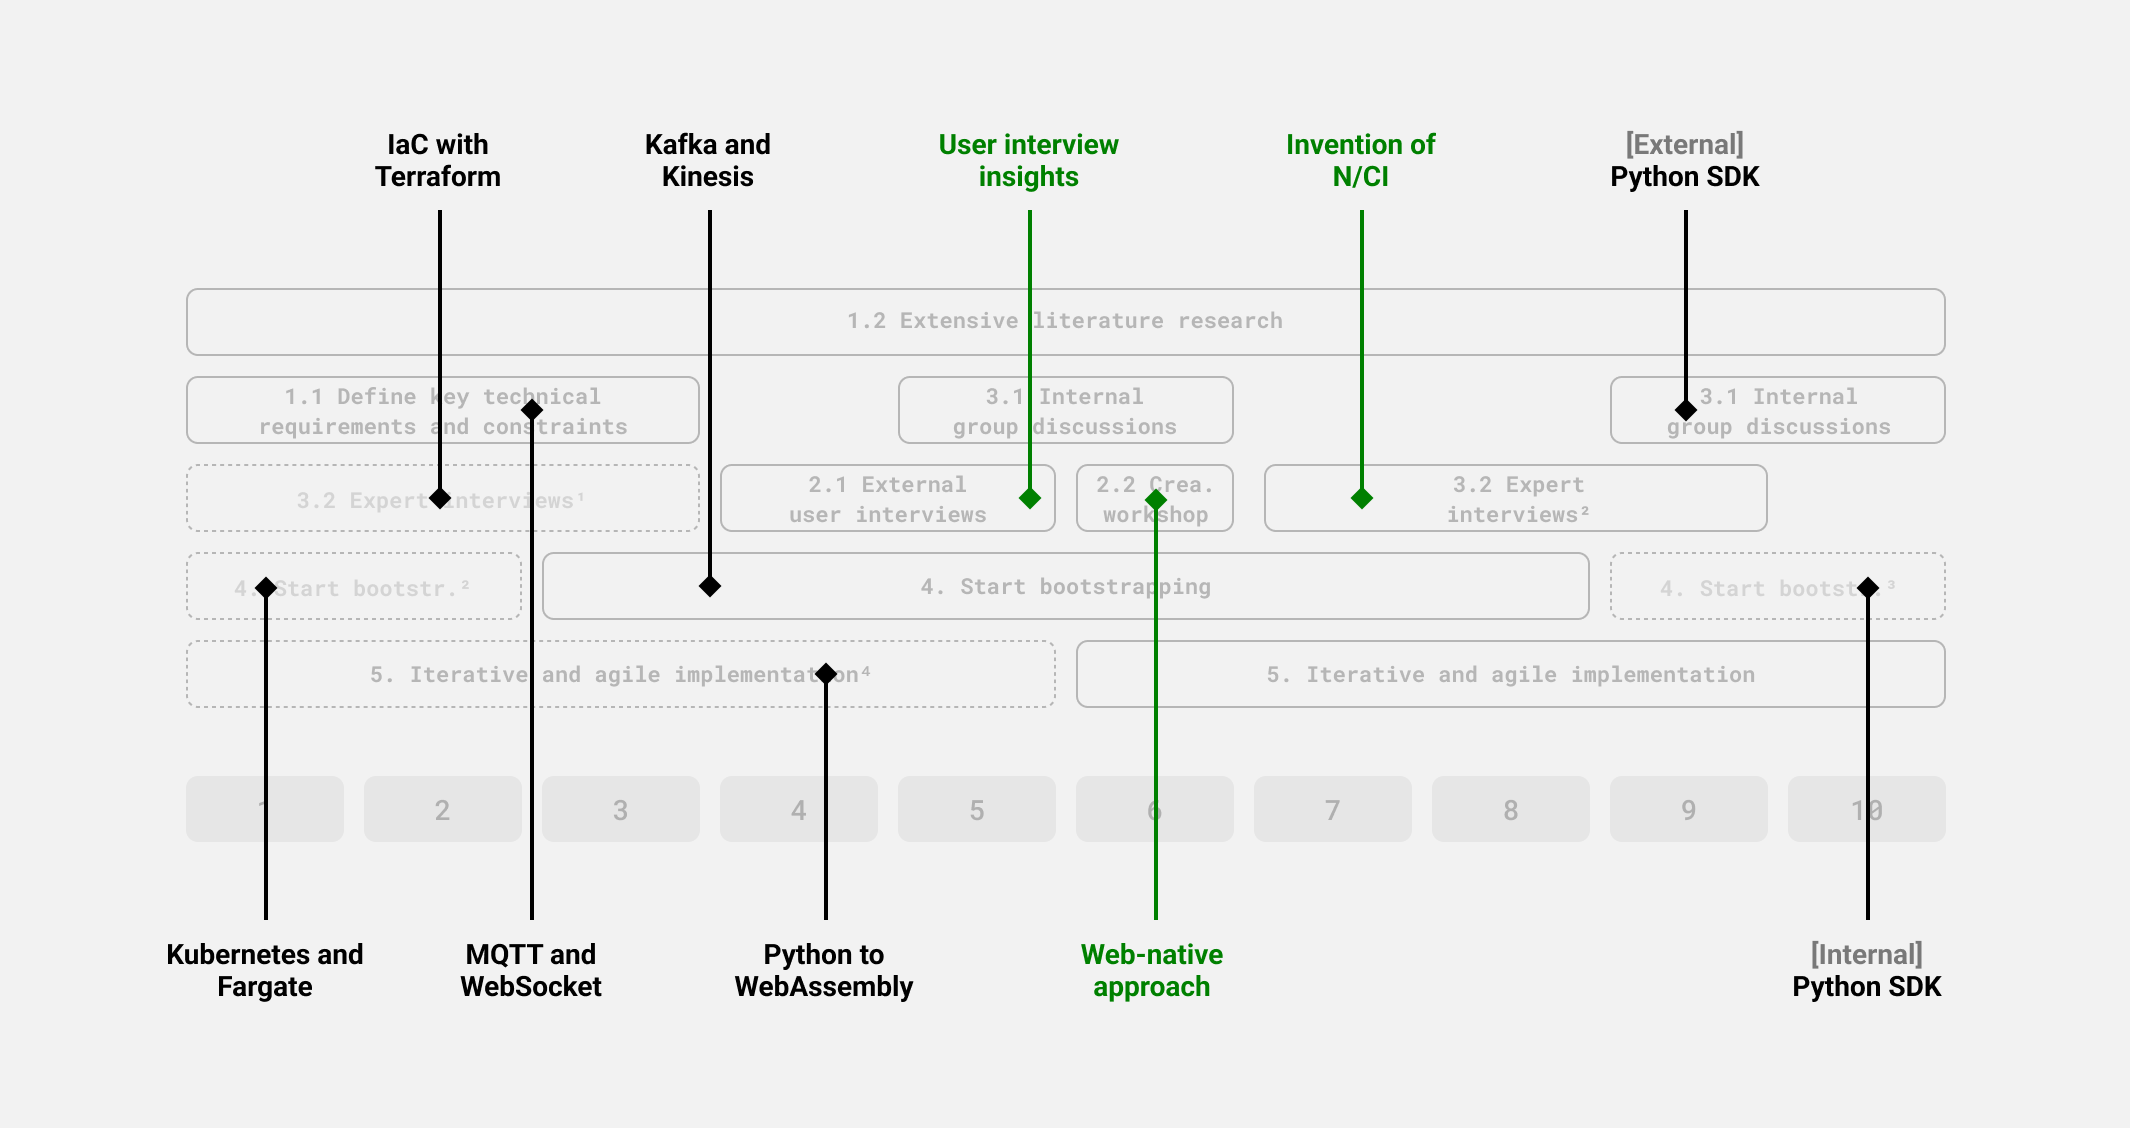
\includegraphics[width=\linewidth]{implementation-timeline-key-events.png}
  \caption{The key events overlaid on the effective project schedule as illustrated in \autoref{fig:implementation-timeline}, with the most influential events coloured green.}
  \label{fig:implementation-timeline-key-events}
\end{figure}

\section{Key events while building a N/CI}
\label{chapter4-key-events}

This section discusses the most influential key event as presented in \autoref{fig:implementation-timeline-key-events} and explains why they occurred as they did and why they were critical to the success of the project. The following outline is not chronologically described but starts with the most significant ones.

\subsection{User interview insights}
\label{chapter4-user-interview-insights}

The conduct of user interviews was one of the most influential key events. This process began with developing customer personas based on the sales team's previous experiences with real customers and the planned customer segments targeted by C-level management. In summary, the author does not want to go into too much detail about how the personas were created and how the process went because the focus is on the results based on the user interviews, not on the persona creation process itself. The personas are illustrated in \autoref{fig:personas}, a descriptive overview of the personas can be found on \autoref{tab:customer-personas} and a more detailed version is included in \autoref{appendix7-other-documents}.

\begin{figure}[!ht]
  \centering
  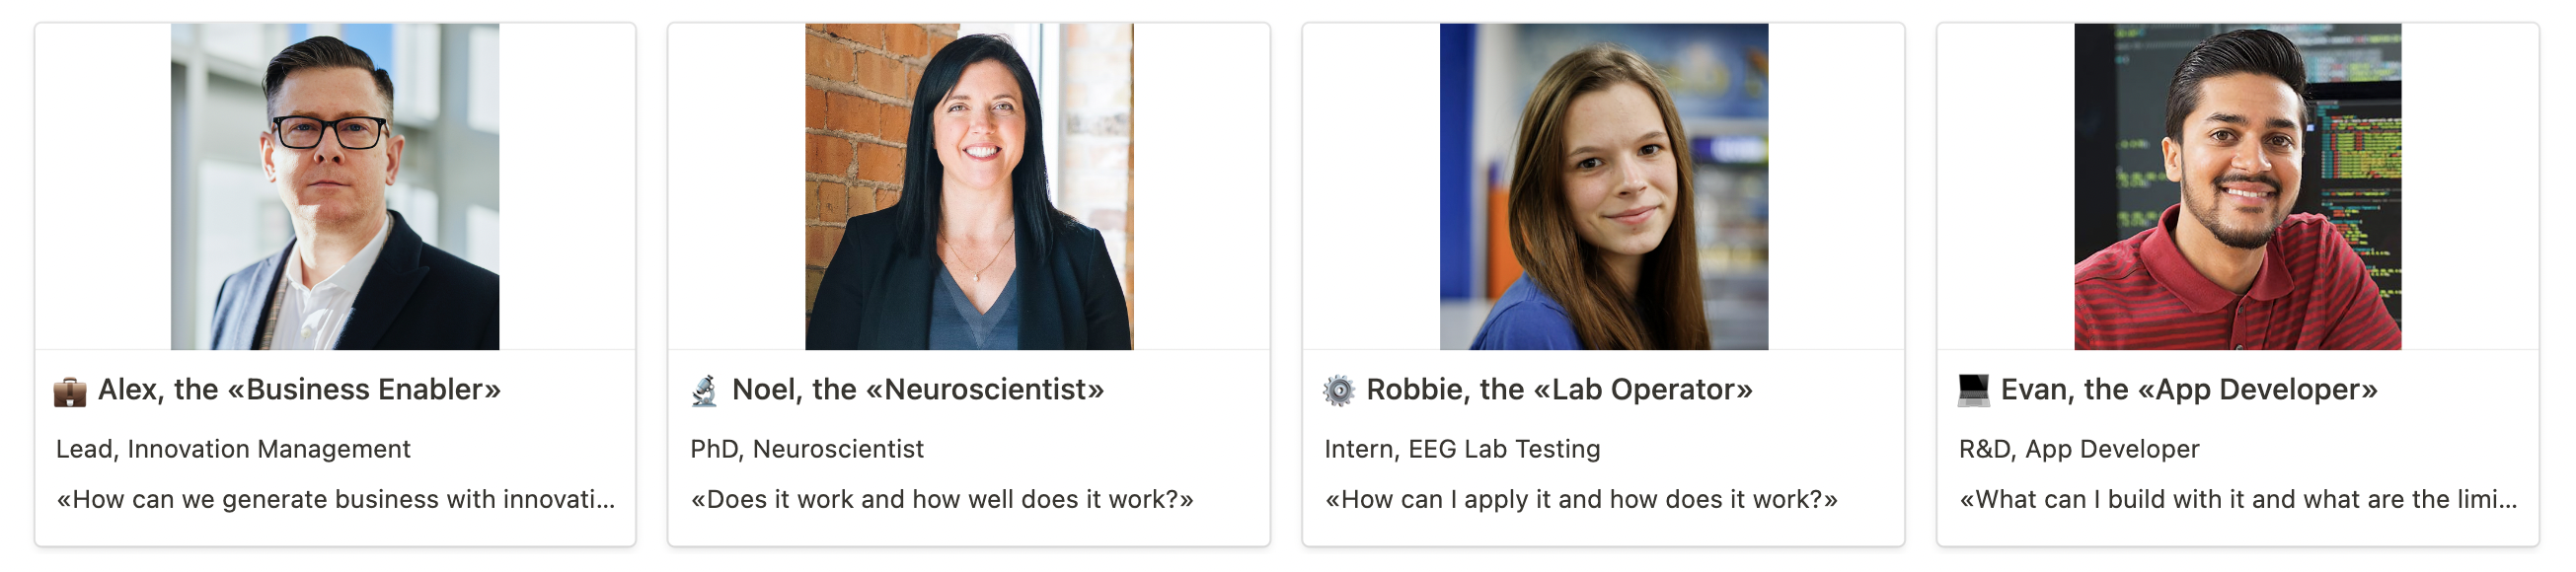
\includegraphics[width=\linewidth]{personas.png}
  \caption[IDUN's customer personas]{IDUN's customer personas \citep{idun_guardian_nodate}.}
  \label{fig:personas}
\end{figure}

\begin{table}[!ht]
  \centering
  \resizebox{\textwidth}{!}{%
    \begin{tabular}{
        >{\columncolor[HTML]{FFFFFF}}l l|l|}
      \cline{3-3}
      \cellcolor[HTML]{000000}{\color[HTML]{FFFFFF} Persona}                  &
      \cellcolor[HTML]{000000}{\color[HTML]{FFFFFF} Occupation}               &
      \cellcolor[HTML]{000000}{\color[HTML]{FFFFFF} Description}                                                                                                                                                                                                                                                                                                                                                                                                                                                                                                                                                                                                                                                                                                                                                                                                                                                                                                                                                                                                                                                                       \\ \hline
      \multicolumn{1}{|l|}{\cellcolor[HTML]{FFFFFF}\textbf{Alex}}             &
      \begin{tabular}[c]{@{}l@{}}Lead,\\ Innovation\\ Management\end{tabular} &
      \begin{tabular}[c]{@{}l@{}}Alex works in a large/small company to bring new innovations and technologies into business\\ and product development roadmaps. Alex informs the company's senior management about new\\ innovations and how they may impact future business and strategic initiatives. Alex has a budget\\ to spend but is supported in decision-making by colleagues in R\&D, product development and\\ innovation scouting.\end{tabular}                                                                                                                                                                                                                                                                                                                                                                                                                                                                                                                                                                                                                                                                           \\ \hline
      \multicolumn{1}{|l|}{\cellcolor[HTML]{FFFFFF}\textbf{Noel}}             &
      \begin{tabular}[c]{@{}l@{}}PhD,\\ Neuroscientist\end{tabular}           &
      \begin{tabular}[c]{@{}l@{}}Noel works within large and small organisations to build innovations based on neuroscience and\\ technologies into future products with an outlook of 5+ years. Noel leads a team or group and\\ informs innovation managers such as Alex about new neurotech products and how they may\\ provide new value to customers. Noel has to get approval to start new projects and obtain\\ budgets for larger initiatives. Noel informs key stakeholders in the organisation and is supported\\ in decision-making by colleagues in R\&D, engineering teams, and innovation scouting.\end{tabular}                                                                                                                                                                                                                                                                                                                                                                                                                                                                                                         \\ \hline
      \multicolumn{1}{|l|}{\cellcolor[HTML]{FFFFFF}\textbf{Robbie}}           &
      \begin{tabular}[c]{@{}l@{}}Intern,\\ EEG Lab Testing\end{tabular}       &
      \begin{tabular}[c]{@{}l@{}}Robbie works within a lab and research group, possibly in large or small organisations, either\\ commercial or academic. Robbie often starts from a study protocol developed with or given by\\ Noel, where a test procedure needs to be followed to have consistent data collection methods\\ with different test subjects. The work of Robbie supports the assumptions and study endpoints\\ or goals defined by Noel and neuroscience colleagues. The results may be used in product\\ development or to prepare a research report, white paper, publication, etc. Robbie works\\ hand-on in the lab, knows how to put on a wet-electrode EEG system, looks at raw signals\\ and understands if the data is being collected correctly. Robbie debugs test setups when things\\ are not running correctly, may process results with scripts and is familiar with lab setups like\\ sleep labs. Robbie can also process the study results, put them together for interpretation\\ together with Noel and support technical details that may (but are not often) communicated\\ to Alex.\end{tabular} \\ \hline
      \multicolumn{1}{|l|}{\cellcolor[HTML]{FFFFFF}\textbf{Evan}}             &
      \begin{tabular}[c]{@{}l@{}}R\&D,\\ App Developer\end{tabular}           &
      \begin{tabular}[c]{@{}l@{}}Evan works within large and small organisations to build engineered solutions based on a\\ toolkit of code and hardware technologies that form the foundations of future products with\\ an outlook of 1-5 years. Evan works in a team or as part of a technical group and works with\\ smart people like Noel. Evan does not have a background in neuroscience but knows about\\ electrical signals and how to build prototypes and demos. Evan needs the approval to spend\\ more than 500 CHF on anything. Evan helps Noel to give great presentations to stakeholders\\ in the organisation but is generally not in strategy discussion. Evan is supported in SCRUM\\ and development tasks by colleagues in the R\&D and engineering teams.\end{tabular}                                                                                                                                                                                                                                                                                                                                         \\ \hline
    \end{tabular}%
  }
  \vspace{10pt}
  \caption{Descriptive overview of IDUN's personas.}
  \vspace{-5pt}
  \label{tab:customer-personas}
\end{table}

People were chosen to represent the personas as accurately as possible. Finally, the author compiled a list of twenty individuals of which seven people were chosen and invited for separate interviews. The interview outline was planned in collaboration with IDUN's product manager and an external industry UX expert, Laura Bendixen, who works as a UX designer at Blick.ch. The author accomplished the outline based on Laura's expertise with previously conducted user interview sessions, which can be found in \autoref{appendix3-user-interviews}. All user interviews were conducted remotely and lasted no more than 1.5 hours. During the interviews, insights were transcribed on post-its. People working with BCIs or EEG were interviewed, as were PhD students working in research labs, developers who, e.g. had never worked with BCIs or had extensive experience building own BCI software, and business enablers from companies responsible, e.g. for BCI-based accessibility. More details about the chosen individual interviewees can be found in \autoref{appendix3-user-interviews}.

The questions were non-leading and open-ended, with the primary goal of allowing interviewees to express themselves, capture their perceptions of the BCI industry, and introduce IDUN's vision and mission upfront. The goal was to determine what software offerings a mass-market BCI product would need to provide, such as convincing developers who have never worked with BCI to include neuro-enhanced features or convincing researchers to use IDUN's NIP in their research. The questions and answers were all about different things. More technically oriented people inquired about speed, performance, and privacy concerns (ergo, more production-readiness thinking), whereas researchers inquired about signal quality, the ability to synchronise with other data streams, and access to raw data (more general applicability thinking). After the last user interview, all post-its were compiled, similar insights were grouped, and the product manager, as well as the author, categorised the most important insights into a list:

\begin{itemize}
  \item There are two prominent use cases: using the NIP for research and developing an end-user-facing app. These are two critical distinctions. Researchers would use the NIP to learn about the brain, such as through simple-setup remote experiments or real-life long-term experiments outside of laboratories. The NIP would, in such a use case, still be used in production, but not to potentially thousands or millions of users in an app intended for end users. The company or developer using the NIP would have physical access to the hardware in the research use case because they would most likely buy one or more devices and hold them in their repertoire. In contrast, companies targeting production use cases would ship the devices as, e.g. white-labelled hardware through their own or 3rd-party channels. Perhaps we can even go so far as to say that because IDUN distributes the device so well, companies and developers do not need to sell the device themselves but can assume that users own such headphones and then access the brain API such as e.g. today's developers can assume that every end-user has GPS access in their smartphone.
  \item Visual demos that are easily accessible for someone owning the hardware are essential for all personas, most notably an Alex. A visual and simple demo should demonstrate what one can do with the NIP from IDUN and inspire others to conduct research, build apps or enable business and opportunities. These demos need to explain to the different personas the different benefits; next to that, the end-user should be able to try out the demos to see the benefits of BCI-enhanced technologies. People like Evan should be able to adapt demos with their codes to create their own versions of them.
  \item The user of the NIP needs to have as low-level control over the data flow and classification as possible but also with an option for less technical users to use it and build things, similar to, e.g. AWS: AWS itself is only an API to use cloud IT resources, but they also have the AWS Console app to build everything via a GUI instead only via the API. What is very important here is that people such as, e.g. Noels need to know precisely what algorithms were used or the methodologies for specific classifiers to justify them and integrate them into their research. They do not, in most instances, actually need raw data access, as plotting functionality would also be enough; therefore, IDUN's NIP should have some functionalities to plot and visualise data.
  \item In order to ease the use of the GUI and the API of the NIP, IDUN needs to provide, next to sufficient documentation, comprehensive libraries for specific environments that make the unobtrusive implementation of the NIP easier. Such as e.g. providing a client-side JavaScript package that is lean and easy to use that can be integrated into existing apps. Examples for such code integration would also need to be provided by IDUN so that people like Evan can easily adjust them and more quickly start integrating them into their apps or research codebases. The personas would need to abstract the brand IDUN as much as possible, e.g. Intel is doing with their Intel-inside ingredient strategy \citep{intel_ingredient_nodate}.
  \item End-users need control over their data so that other companies accessing the NIP API cannot collect their data on their servers and do everything they want. Imagine if, e.g. the operating system layer of one's smartphone would not offer an opt-in mechanism for the cameras, then 3rd-party developers could install spyware and record without the user permits it. When, e.g. users start to use multiple apps with a NIP integration, there needs to be some way to control the opt-in and data access without the app developers having any saying on the decisions. There needs to be a technical limitation from the side of the hardware or the cloud to ensure user privacy and data security for end-users.
  \item Researchers are very interested in the raw EEG data and the synchronisation possibilities with specific protocols such as LSL to combine, e.g. a heart rate sensor with the EEG collected from IDUN's hardware. The NIP software offering needs to give enough freedom to combine the data without letting all other collected data flow into the NIP from IDUN. This means that the NIP should be able to collect, transform and, most importantly, label data in correlation with other data streams with a local option to satisfy researchers like Noel.
\end{itemize}

These insights were critical in determining that there must be sufficient freedom for raw data research without releasing raw data into mass market production environments to protect end-user privacy. As a result, an opt-in mechanism outside of third-party ecosystems is required. A library that can be implemented in end-user apps and connects directly to the hardware without the need to download a companion app from IDUN itself is also required. This library should allow researchers to access it locally and, e.g. use their preferred protocols to synchronise tags and labels with other data streams. Nonetheless, IDUN's NIP should once again provide some control over how much raw data can be collected and restrict access if, e.g. the proposed research project or experiment time frame is exceeded. Furthermore, additional NIP functions should be added to visualise easy-to-use demos for all personas, as well as a way to use and control the NIP without having to write code, but with enough flexibility and transparency that there is trust in the system and even advanced users can work with a visual tool instead of code.

\subsection{Invention of N/CI}
\label{chapter4-invention-of-nci}

The insights from the user interviews, combined with the ongoing research on B/CI and remote BCI mentioned in the introduction chapter, were key to realising the novelty of this new interdisciplinary approach to developing a production-grade and mass-market BCI software system running in the cloud and targeting the general population via general applicability. It is important to note that the realisation that such a system had not yet been defined in research only emerged in the seventh sprint. The findings from the user interviews were primarily in the direction of the N/CI definition, while the literature review was primarily in the direction of distinguishing between existing research and definitions.

Once a first draft of the definition was written down, the research and separation of work packages could be more easily tackled and explored due to a better understanding of what was new and unexplored. At the time of the end of the seventh sprint, the author's goal was to develop further and define the definition and motivation in the form of an written appendix (\autoref{appendix1-definition-and-motivation-of-a-nci}) to attach to the context chapter of this thesis.

\section*{Web-native approach}
\label{chapter4-web-native-approach}

Before Sprint 6, there were some ideas about future architecture roadmaps designed by the author of this thesis, as shown on \autoref{fig:architecture-roadmap}.

\begin{figure}[!ht]
  \centering
  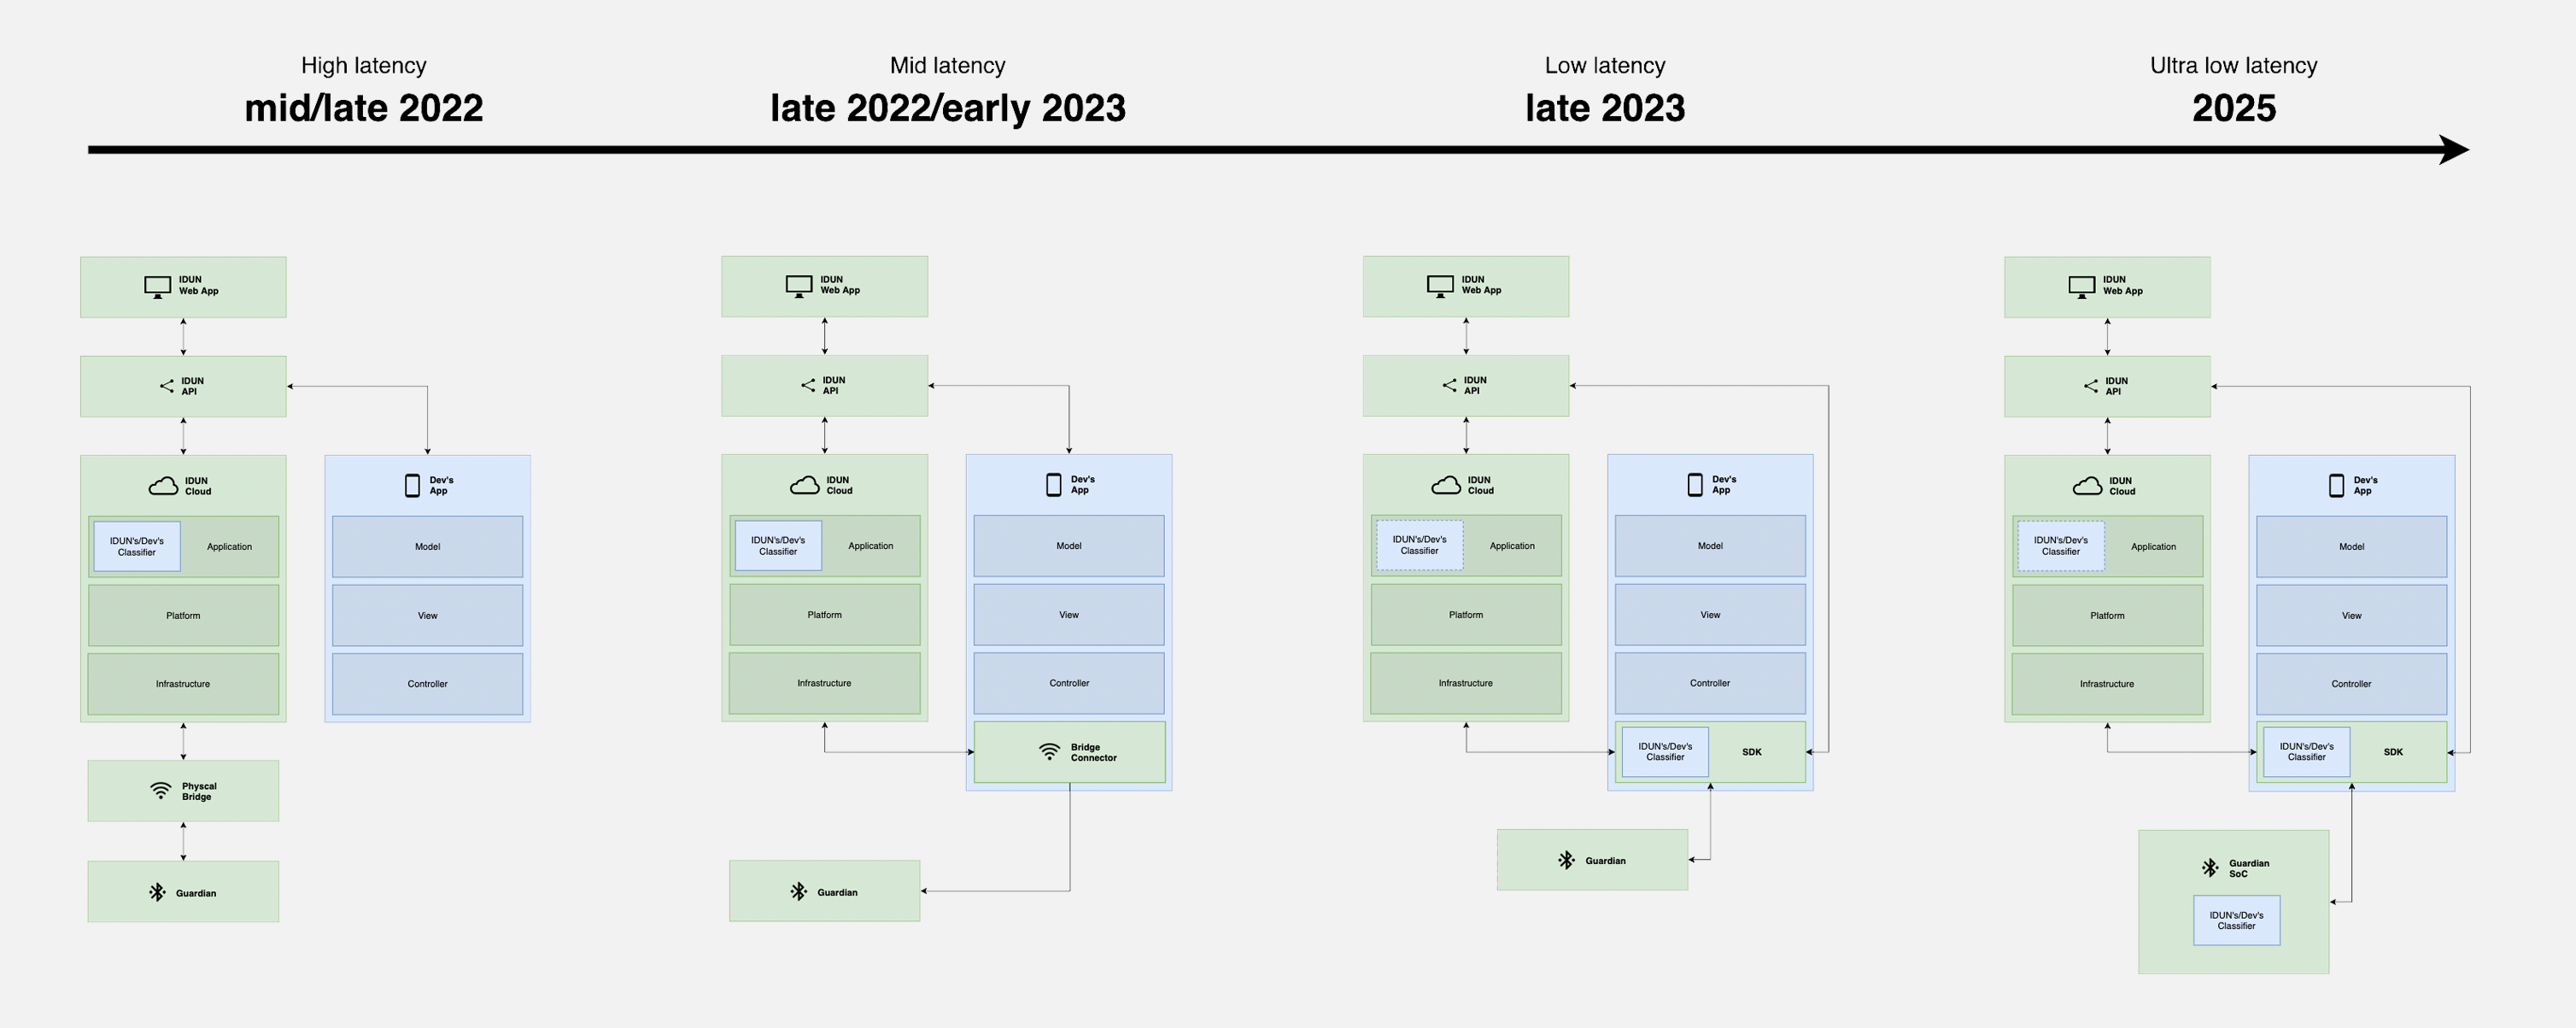
\includegraphics[width=\linewidth]{architecture-roadmap.png}
  \caption{Original architecture roadmap of IDUN's NIP going from a high latency system in mid/late 2022 to a ultra low latency system in 2025.}
  \label{fig:architecture-roadmap}
\end{figure}

The initial architecture roadmap was part of the project's initial phase to define the key technical requirements and constraints and show how the NIP software stack would move from a high latency system to a low latency system. Nonetheless, one aspect of this old architecture roadmap was that IDUN would continue to maintain and develop the physical hardware network bridge and eventually port it to end-user devices as a companion app. However, just before Sprint 6, the author stumbled upon the work of \citeauthor{flynn_brainsplay_nodate} of the BCI platform called Brains at Play and its use of Web Bluetooth \citep{brainsplay_add_nodate}, which is a new and experimental API for browsers that allows websites to connect directly to a Bluetooth Low Energy (BLE) device. The Brains at Play platform is a hardware-independent BCI software platform with similar goals to Neuromore Studio. The main difference is that they offer their app as a web app; therefore, everything runs in the browser without downloading additional software. The author contacted Garrett Flynn, one of the founding partners, and discussed the implications and findings of using Web Bluetooth, e.g. EEG data such as that from IDUN's sensor (later, Garrett Flynn was also invited to the user interviews as one of the persona representatives for Evan). Garrett Flynn's findings were entirely positive, and he strongly recommended working with the API as it makes deploying a BCI platform much more effortless than deploying applications for any operating system, especially any BLE interface. However, one of the main disadvantages of Web Bluetooth was browser compatibility, as shown in \autoref{fig:can-i-use}.

\begin{figure}[!ht]
  \centering
  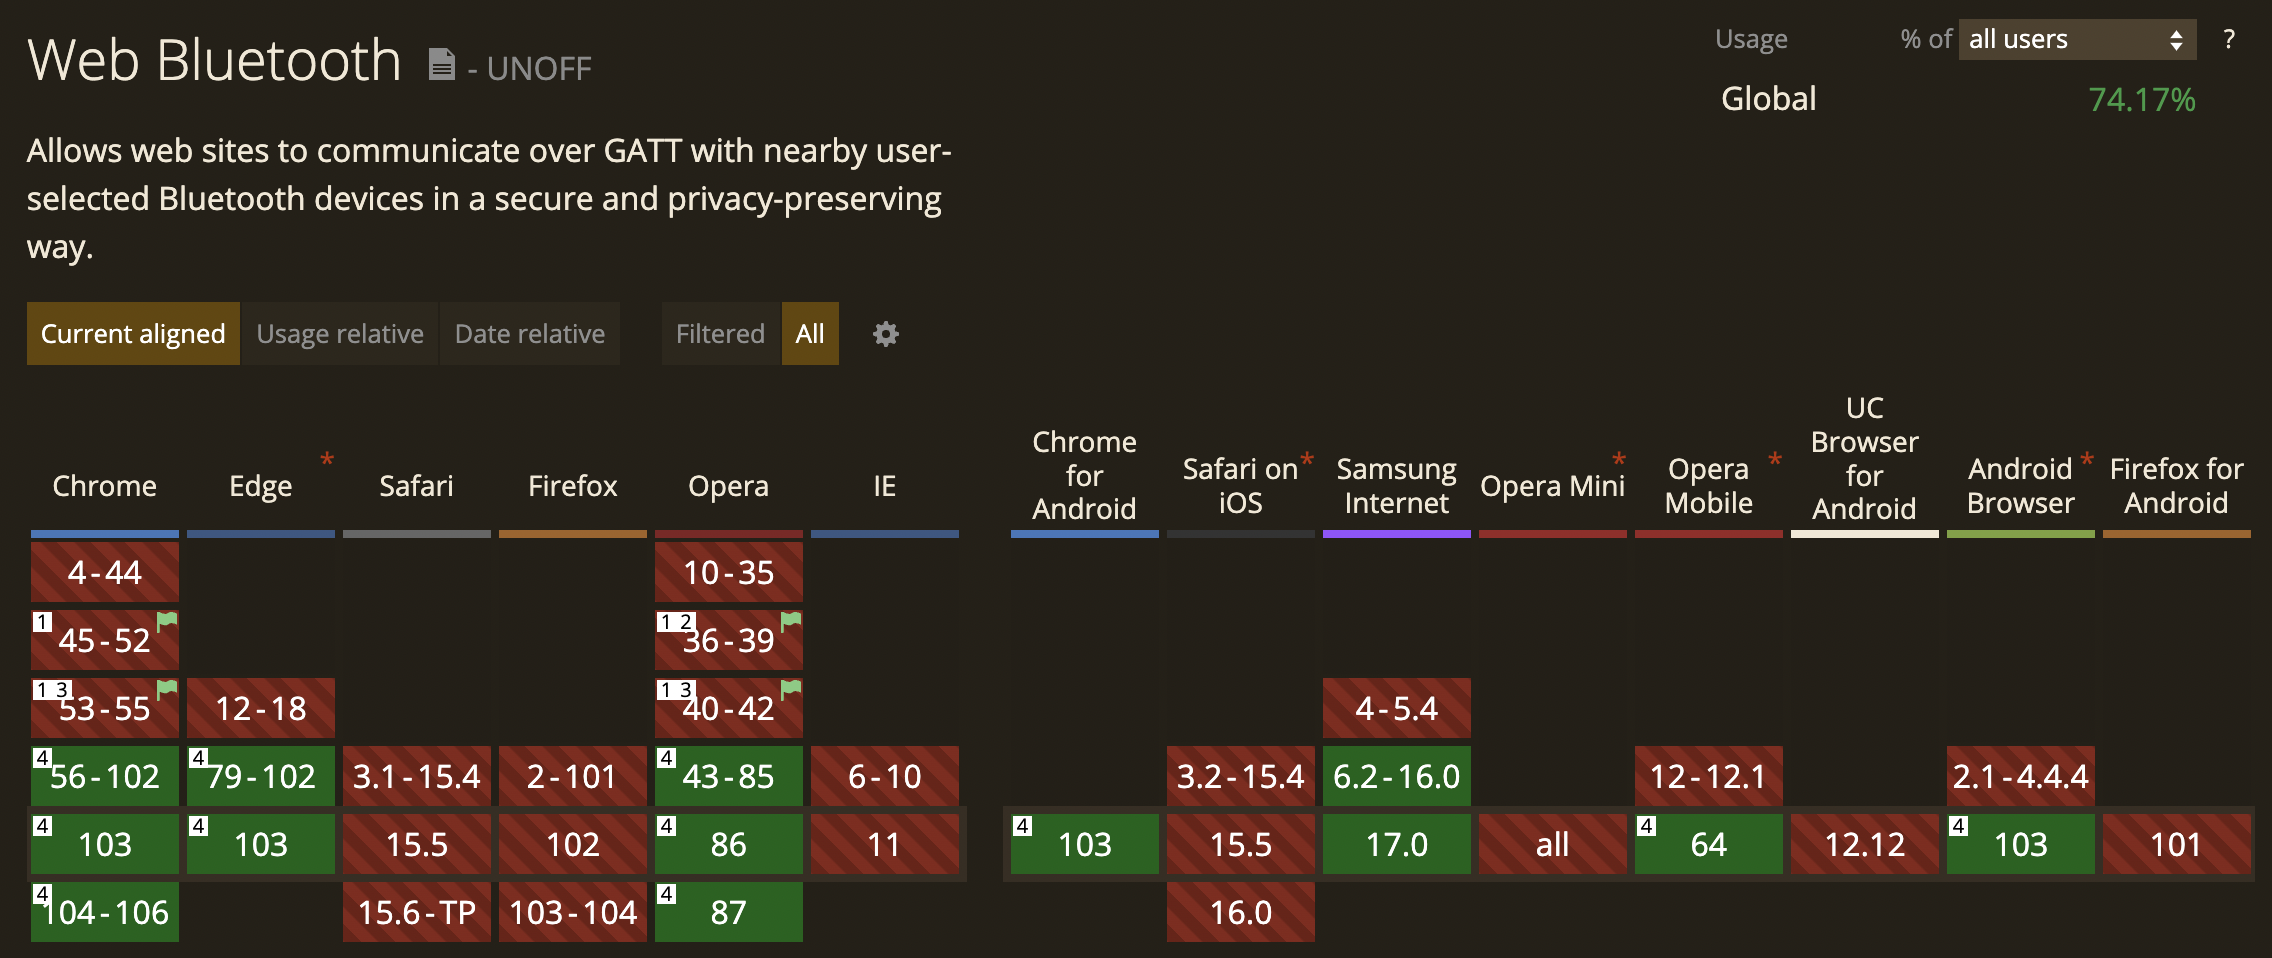
\includegraphics[width=\linewidth]{can-i-use.png}
  \caption[Browser compatibility overview of Web Bluetooth]{Browser compatibility overview of Web Bluetooth \citep{caniuse_web_nodate}.}
  \label{fig:can-i-use}
\end{figure}

Nevertheless, IDUN is building a product that aims for an extensive user base in 2-3 years, as can be seen on their roadmap in \autoref{fig:idun-timeline}. This means that browser compatibility could come and ease out over the coming years once browser manufacturers start implementing the API. One problem, however, is that the Web Bluetooth API cannot be run in a service worker, making it impossible to run in the background when e.g. the device has its screen locked or another app is currently opened on a smartphone \citep{webbluetoothcg_service_2018}, which is an intermediate problem, even for the upcoming smaller and specific user groups with the current personas. Among a variety of technologies under investigation, the author identified Capacitor, a JavaScript library, to be a suitable candidate for the current use case. It essentially can compile and run web apps as native apps, with the ability to access native APIs \citep{ionic_capacitor_nodate}, such as the camera or, especially important for IDUN, the BLE API \citep{capacitor-community_capacitor-communitybluetooth-_2022}. Developers can use Capacitor to write BLE code with the same interface as Web Bluetooth, compile the code and run the applications on native devices with background functionality.

After further research, as shown in \autoref{appendix7-other-documents}, almost the entire Sprint 6 was spent evaluating the possibility of using Web Bluetooth for IDUN's NIP. At the end of the sprint, a working PoC SPA was created with an iOS and Android build that fulfilled all needs in terms of developer experience, the latency of the EEG signal from the device to a visualisation plot and the power consumption of lower-end smartphones. Following this, the author proposed to change the original architecture roadmap as depicted on \autoref{fig:architecture-roadmap} and skip the first two steps and go directly to step 3 in order to accelerate the development pace and enable greater market maturity for IDUN's NIP as soon as the end of 2022.

The use of a web app, combined with the use of modern APIs and the compilation of the app for mobile applications when compatibility is not guaranteed, is called a web-native approach \citep{ionic_web_nodate}. Besides the time saved by not having to develop platform-specific apps but using a single code base, this approach also has the advantage that a library that abstracts the logic of connecting a BLE device such as the IDUN device can already be created into a single installable unit, e.g. in the form of an NPM package. This library can be implemented in end-user apps and connects directly to the hardware without the need to download a companion app from IDUN itself, and is one of the solutions to the findings from the user interviews. The time saved with a web-native approach allowed IDUN to already focus on creating such a library and using it in their web app, which would be the console or GUI as in the AWS example, allowing dogfooding for IDUN's own software offerings and eliminating preliminary issues before releasing the library to the public \citep{techopedia_what_2016}.

Further key events of the case study as displayed in black text depicted in \autoref{fig:implementation-timeline-key-events} are described in more detail in \autoref{appendix4-further-key-events}.

\nomenclature[ble]{BLE}{Bluetooth Low Energy}
\nomenclature[eks]{EKS}{Elastic Kubernetes Service}
\nomenclature[s3]{S3}{Simple Storage Service}
\nomenclature[rest]{REST}{Representational state transfer}
\nomenclature[cdk]{CDK}{Cloud Development Kit}
\nomenclature[cicd]{CI/CD}{Continuous integration and continuous delivery}
